\chapter{Periodic Structure of Crystals}
\section{Bravais lattices}
\dfn{Bravais latticees}{There are 14 different lattice types, these are called Bravais lattices. These lattices can be subdivided into 7 different lattice systems, these lattice systems are:
\begin{enumerate}
    \setlength\itemsep{0pt}
    \item   Triclinic
    \item   Monoclinic
    \item   Orthohombric
    \item   Tetragonal
    \item   Cubic
    \item   Triagonal
    \item   Hexagonal
\end{enumerate}
The Cubic structure will mostly be studied during this course.
}

\section{Cubic lattice systems}
Cubic lattice systems come in three flavours, we will define them here. The different systems can be found in figure \ref{fig:cubic_lattice_systems}.
\begin{figure}
    \centering
    \begin{tikzpicture}
		%	Bottom front
		\filldraw [black]	(0, 0) circle (2pt);
		\draw [-*, black]	(0, 0) to (1, 0);

		%	Top front
		\filldraw [black]	(0, 1) circle (2pt);
		\draw [-*, black]	(0, 1) to (1, 1);

		%	Horzontal front
		\draw[--, black]	(0, 0) to (0, 1)
							(0.9, 0) to (0.9, 1);

		%	Top oblique
		\draw[-*, black]	(0, 1) to (0.55, 1.5);
		\draw[-*, black]	(0.9, 1) to (1.45, 1.5);

		%	Side right
		\draw[-*, black]	(1.4, 1.5) to (1.4, 0.4);
		\draw[--, black]	(0.9, 0) to (1.4, 0.5);

		%	Top back
		\draw[--, black]	(0.4, 1.45) to (1.4, 1.45);

		%	Inside
		\draw[dotted, black]	(0.5, 0.5) to (1.4, 0.5)
                                (0.5, 0.5) to (0, 0)
								(0.5, 1.5) to (0.5, 0.5);
		\filldraw[black]	(0.5, 0.5) circle (1pt);

 		\draw [<->, black, thick]	(0, -0.3) to node [below] {a} (0.9, -0.3);
 		\draw [<->, black, thick]	(1.7, 0.5) to node [right] {a} (1.7, 1.5);
 		\draw [<->, black, thick]	(1.1, -0.1) to node [below=1mm] {a} (1.6, 0.4);
	\end{tikzpicture}
%
	\begin{tikzpicture}
		%	Bottom front
		\filldraw [black]	(0, 0) circle (2pt);
		\draw [-*, black]	(0, 0) to (1, 0);

		%	Top front
		\filldraw [black]	(0, 1) circle (2pt);
		\draw [-*, black]	(0, 1) to (1, 1);

		%	Horzontal front
		\draw[--, black]	(0, 0) to (0, 1)
							(0.9, 0) to (0.9, 1);

		%	Top oblique
		\draw[-*, black]	(0, 1) to (0.55, 1.5);
		\draw[-*, black]	(0.9, 1) to (1.45, 1.5);

		%	Side right
		\draw[-*, black]	(1.4, 1.5) to (1.4, 0.4);
		\draw[--, black]	(0.9, 0) to (1.4, 0.5);

		%	Top back
		\draw[--, black]	(0.4, 1.45) to (1.4, 1.45);

		%	Inside
		\draw[dotted, black]	(0.5, 0.5) to (1.4, 0.5)
                                (0.5, 0.5) to (0, 0)
								(0.5, 1.5) to (0.5, 0.5);
		\filldraw[black]	(0.5, 0.5) circle (1pt);

		% Body centering
		\filldraw [gray] (0.7, 0.7) circle (2pt);

 		\draw [<->, black, thick]	(0, -0.3) to node [below] {a} (0.9, -0.3);
 		\draw [<->, black, thick]	(1.7, 0.5) to node [right] {a} (1.7, 1.5);
 		\draw [<->, black, thick]	(1.1, -0.1) to node [below=1mm] {a} (1.6, 0.4);
	\end{tikzpicture}
%
	\begin{tikzpicture}
		%	Face centering
		\filldraw [gray]	(0.95, 0.95) circle (2pt);

		%	Bottom front
		\filldraw [black]	(0, 0) circle (2pt);
		\draw [-*, black]	(0, 0) to (1, 0);

		%	Top front
		\filldraw [black]	(0, 1) circle (2pt);
		\draw [-*, black]	(0, 1) to (1, 1);

		%	Horzontal front
		\draw[--, black]	(0, 0) to (0, 1)
							(0.9, 0) to (0.9, 1);

		%	Top oblique
		\draw[-*, black]	(0, 1) to (0.55, 1.5);
		\draw[-*, black]	(0.9, 1) to (1.45, 1.5);

		%	Side right
		\draw[-*, black]	(1.4, 1.5) to (1.4, 0.4);
		\draw[--, black]	(0.9, 0) to (1.4, 0.5);

		%	Top back
		\draw[--, black]	(0.4, 1.45) to (1.4, 1.45);

		%	Inside
		\draw[dotted, black]	(0.5, 0.5) to (1.4, 0.5)
                                (0.5, 0.5) to (0, 0)
								(0.5, 1.5) to (0.5, 0.5);
		\filldraw[black]	(0.5, 0.5) circle (1pt);

		% Face centering
		\filldraw [gray]	(0.5, 0.5) circle (2pt)
							(0.25, 0.75) circle (2pt)
							(0.7, 1.25) circle (2pt)
 							(0.7, 0.25) circle (2pt)
 							(1.15, 0.7) circle (2pt);

 		\draw [<->, black, thick]	(0, -0.3) to node [below] {a} (0.9, -0.3);
 		\draw [<->, black, thick]	(1.7, 0.5) to node [right] {a} (1.7, 1.5);
 		\draw [<->, black, thick]	(1.1, -0.1) to node [below=1mm] {a} (1.6, 0.4);
	\end{tikzpicture}
    \caption{The three different cubic lattice systems}
    \label{fig:cubic_lattice_systems}
\end{figure}
\dfn{Simple cubic lattice}{A simple cubic lattice is a conventional unit cell and therefore also a \textit{PUC}. This lattice has a straightforward basis, as can be seen in figure \ref{fig:simple_cubic_lattice}.}
The basis chosen is $\{\vec{a}_1, \vec{a}_2, \vec{a}_3\}$. As we can see (figure \ref{fig:simple_cubic_lattice}), the basis isn't body centered. Because the body centered atom is a different one as the other 'side' atoms, the smallest possible unit cell (or \textit{PUC}) is the full cube. Whereas if the middle atom is the same, the basis is chosen in the middle, this is the \textbf{body centered cubic lattice}.
\begin{figure}[h]
    \centering
    \begin{tikzpicture}
		%	Bottom front
		\filldraw [black]	(0, 0) circle (2pt);
		\draw [-*, black]	(0, 0) to (1, 0);

		%	Top front
		\filldraw [black]	(0, 1) circle (2pt);
		\draw [-*, black]	(0, 1) to (1, 1);

		%	Horzontal front
		\draw[--, black]	(0, 0) to (0, 1)
							(0.9, 0) to (0.9, 1);

		%	Top oblique
		\draw[-*, black]	(0, 1) to (0.55, 1.5);
		\draw[-*, black]	(0.9, 1) to (1.45, 1.5);

		%	Side right
		\draw[-*, black]	(1.4, 1.5) to (1.4, 0.4);
		\draw[--, black]	(0.9, 0) to (1.4, 0.5);

		%	Top back
		\draw[--, black]	(0.4, 1.45) to (1.4, 1.45);

		%	Inside
		\draw[dotted, black]	(0.5, 0.5) to (1.4, 0.5)
                                (0.5, 0.5) to (0, 0)
								(0.5, 1.5) to (0.5, 0.5);
		\filldraw[black]	(0.5, 0.5) circle (1pt);

		% Body centering
		\filldraw [cyan] (0.7, 0.7) circle (2pt);

		\draw [->, cyan, thin]	(0.7, 0.7) to node [right=9mm]{different atom} (2.4, 0.7);

 		\draw [<->, black, thick]	(0, -0.3) to node [below] {a} (0.9, -0.3);
 		\draw [<->, black, thick]	(1.7, 0.5) to node [right] {a} (1.7, 1.5);
 		\draw [<->, black, thick]	(1.1, -0.1) to node [below=1mm] {a} (1.6, 0.4);

 		%	Basis
 		\draw [|->, green, very thick]	(0, 0) to (0.9, 0);
 		\draw [|->, red, very thick]	(0, 0) to (0, 1);
 		\draw [|->, blue, very thick]	(0, 0) to (0.48, 0.48);
	\end{tikzpicture}
	\caption{The basis for a simple cubic lattice}
	\label{fig:simple_cubic_lattice}
\end{figure}

\dfn{Body centered cubic lattice}{A Body centered cubic lattice has 1 atom as primitive unit cell, its basis is depectied in figure \ref{fig:bodycubic_lattice_system}. As mentioned before, all atoms are the same and that is why the \textit{PUC} is smaller.}
\begin{figure}[h]
    \centering
	\begin{tikzpicture}
		%	Bottom front
		\filldraw [black]	(0, 0) circle (2pt);
		\draw [-*, black]	(0, 0) to (1, 0);

		%	Top front
		\filldraw [black]	(0, 1) circle (2pt);
		\draw [-*, black]	(0, 1) to (1, 1);

		%	Horzontal front
		\draw[--, black]	(0, 0) to (0, 1)
							(0.9, 0) to (0.9, 1);

		%	Top oblique
		\draw[-*, black]	(0, 1) to (0.55, 1.5);
		\draw[-*, black]	(0.9, 1) to (1.45, 1.5);

		%	Side right
		\draw[-*, black]	(1.4, 1.5) to (1.4, 0.4);
		\draw[--, black]	(0.9, 0) to (1.4, 0.5);

		%	Top back
		\draw[--, black]	(0.4, 1.45) to (1.4, 1.45);

		%	Inside
		\draw[dotted, black]	(0.5, 0.5) to (1.4, 0.5)
                                (0.5, 0.5) to (0, 0)
								(0.5, 1.5) to (0.5, 0.5);
		\filldraw[black]	(0.5, 0.5) circle (1pt);

		% Body centering
		\filldraw [gray] (0.7, 0.7) circle (2pt);

 		\draw [<->, black, thick]	(0, -0.3) to node [below] {a} (0.9, -0.3);
 		\draw [<->, black, thick]	(1.7, 0.5) to node [right] {a} (1.7, 1.5);
 		\draw [<->, black, thick]	(1.1, -0.1) to node [below=1mm] {a} (1.6, 0.4);

 		%	Basis
 		\draw [|->, green, very thick]	(0.7, 0.7) to (0.05, 0.05);
 		\draw [|->, red, very thick]	(0.7, 0.7) to (1.4, 0.5);
 		\draw [|->, blue, very thick]	(0.7, 0.7) to (1, 1);
	\end{tikzpicture}
    \caption{The three different cubic lattice systems}
    \label{fig:bodycubic_lattice_system}
\end{figure}

\dfn{Face centered cubic lattice}{If all atoms are the same and the extra atoms position themselves on the middle of every face, one gets the face centere cubic lattice. This is depicted in figure \ref{fig:facecubic_lattice_system}.}
\begin{figure}[h]
    \centering
	\begin{tikzpicture}
		%	Face centering
		\filldraw [gray]	(0.95, 0.95) circle (2pt);

		%	Bottom front
		\filldraw [black]	(0, 0) circle (2pt);
		\draw [-*, black]	(0, 0) to (1, 0);

		%	Top front
		\filldraw [black]	(0, 1) circle (2pt);
		\draw [-*, black]	(0, 1) to (1, 1);

		%	Horzontal front
		\draw[--, black]	(0, 0) to (0, 1)
							(0.9, 0) to (0.9, 1);

		%	Top oblique
		\draw[-*, black]	(0, 1) to (0.55, 1.5);
		\draw[-*, black]	(0.9, 1) to (1.45, 1.5);

		%	Side right
		\draw[-*, black]	(1.4, 1.5) to (1.4, 0.4);
		\draw[--, black]	(0.9, 0) to (1.4, 0.5);

		%	Top back
		\draw[--, black]	(0.4, 1.45) to (1.4, 1.45);

		%	Inside
		\draw[dotted, black]	(0.5, 0.5) to (1.4, 0.5)
                                (0.5, 0.5) to (0, 0)
								(0.5, 1.5) to (0.5, 0.5);
		\filldraw[black]	(0.5, 0.5) circle (1pt);

		% Face centering
		\filldraw [gray]	(0.5, 0.5) circle (2pt)
							(0.25, 0.75) circle (2pt)
							(0.7, 1.25) circle (2pt)
 							(0.7, 0.25) circle (2pt)
 							(1.15, 0.7) circle (2pt);

 		\draw [<->, black, thick]	(0, -0.3) to node [below] {a} (0.9, -0.3);
 		\draw [<->, black, thick]	(1.7, 0.5) to node [right] {a} (1.7, 1.5);
 		\draw [<->, black, thick]	(1.1, -0.1) to node [below=1mm] {a} (1.6, 0.4);

 		%	Basis
 		\draw [|->, red, very thick]	(0, 0) to (0.25, 0.75);
 		\draw [|->, blue, very thick]	(0, 0) to (0.7, 0.25);
		\draw [|->, green, very thick]	(0, 0) to (0.5, 0.5);
	\end{tikzpicture}
    \caption{The three different cubic lattice systems}
    \label{fig:facecubic_lattice_system}
\end{figure}

\section{C/Si/Ge - lattice systems}
As we know, the lattice systems for C, Si and Ge have a diamond lattice structre. This diamond structure takes the form of a fcc (face centered cubic) lattice. In figure \ref{fig:diamondstruct}, one can see the primitive unit cell. The basis vectors are:
\begin{align}
	\vec{a}_1 &= (\frac{1}{2}, \frac{1}{2}, 0) \\
	\vec{a}_2 &= (0, \frac{1}{2}, \frac{1}{2}) \\
	\vec{a}_3 &= (\frac{1}{2}, 0, \frac{1}{2})
\end{align}

\begin{figure}
	\centering
	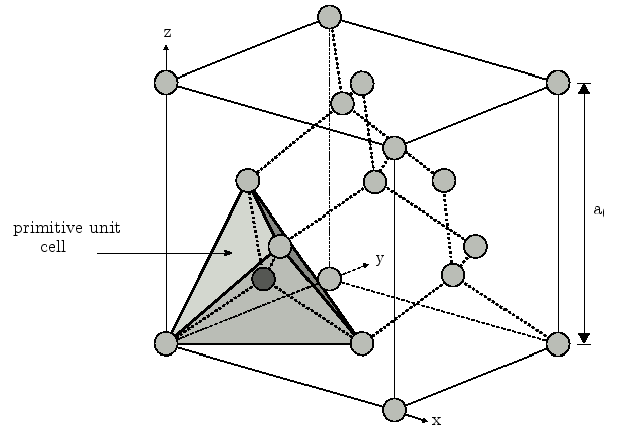
\includegraphics[width=\textwidth/2]{./diamondstructure}
	\caption{The diamond structure and its \textit{PUC}}
	\label{fig:diamondstruct}
\end{figure}

\subsection{Translation symmetry} \label{sec:trans_symm}
As a tiny intermezzo I'll introduce tranlation symmetry. This will be important later on for solving the Schrödinger equation.
\begin{align}
	& \left\{-\frac{\hbar}{2m}\nabla^2 + V(\vec{r})\right\}\phi(\vec{r}) = E\phi(\vec{r}) \\
	& \qquad \longrightarrow V(\vec{r} + \vec{T}) = V(\vec{r}') = V(\vec{r})
\end{align}
Because $V(\vec{r})$ is actually a periodic function in a crystal lattice, it becomes $V(\vec{r} + \vec{T})$. This $\vec{T}$ is responsible for the translation in translational symmetry.
\dfn{Translational symmetry}{Translational symmetry is a symmetry operation for a crystal. This operation leaves the crystal invariant. Meaning that the addition of $\vec{T}$ to $\vec{r}$ returns the same value for $V(\vec{r})$. This is graphically represented in figure \ref{fig:trans_symm}.}

\begin{figure}
	\centering
	\begin{tikzpicture}
		\draw [->, black]	(0, 0, 0) to (0, 0, 4) node[anchor=north east]{$x$};
		\draw [->, black]	(0, 0, 0) to (0, 4, 0) node[above]{$z$};
		\draw [->, black]	(0, 0, 0) to (4, 0, 0) node[right]{$y$};

		\draw [->, blue, very thick]	(0, 0, 0) to (4, 3, 2) node[left=5mm]{$\vec{r}$};
		\draw [->, green, very thick]	(4, 3, 2) to (5, 2, 2) node[above=3mm]{$\vec{T}$};
		\draw [->, red, very thick]		(0, 0, 0) to (5, 2, 2) node[left=5mm]{$\vec{r}'$}
	\end{tikzpicture}
	\caption{Translational symmetry}
	\label{fig:trans_symm}
\end{figure}

\section{Lattice dimensions}
\dfn{Lattice dimensions}{Lattice dimensions are defined by the parameters [$u, v, w$]. These parameters are defined by a vector $\vec{r} = k(u\vec{a}_1 + v\vec{a}_2 + w\vec{a}_3)$. \\
$\vec{a}_1, \vec{a}_2, \vec{a}_3$ are unit cell vectors, $k$ is a common factor in order that $u, v, w \in \bbZ_{without\, common\, factor}$. \\
One thing to notice is that if $\vec{a}_1, \vec{a}_2, \vec{a}_3$ are \textit{PLV}s, $k \in \bbZ$. Else $k \in \bbQ$.}
\ex{Lattice dimensions}{
Take the following vector in the lattice:

\begin{center}
	\begin{tikzpicture}
		\draw [->, gray]	(0, 0, 0) to (0, 0, 4) node[anchor=north east]{$x$};
		\draw [->, gray]	(0, 0, 0) to (0, 4, 0) node[above]{$z$};
		\draw [->, gray]	(0, 0, 0) to (4, 0, 0) node[right]{$y$};

		\draw [->, blue, very thick]	(0, 0, 0) to (1.95, 1.95, 0);

		\filldraw [gray]	(0, 0, 0) circle (2pt);

		\draw [dotted, black]	(0, 0, 0) to (0, 0, 2);
		\draw [dotted, black]	(0, 0, 0) to (0, 2, 0);
		\draw [dotted, black]	(0, 0, 0) to (2, 0, 0);

		\draw [-, black]	(2, 0, 0) to (2, 0, 2);
		\draw [-, black]	(0, 0, 2) to (2, 0, 2);

		\draw [-, black]	(0, 0, 2) to (0, 2, 2);
		\draw [-, black]	(2, 0, 2) to (2, 2, 2);
		\draw [-, black]	(2, 0, 0) to (2, 2, 0);

		\draw [-, black]	(0, 2, 0) to (0, 2, 2);
		\draw [-, black]	(0, 2, 2) to (2, 2, 2);
		\draw [-, black]	(2, 2, 0) to (2, 2, 2);
		\draw [-, black]	(0, 2, 0) to (2, 2, 0);

		\filldraw	(0, 2, 0) circle (2pt)
					(2, 0, 2) circle (2pt)
					(2, 0, 0) circle (2pt)
					(2, 2, 2) circle (2pt)
					(0, 2, 2) circle (2pt)
					(2, 2, 0) circle (2pt)
					(0, 0, 2) circle (2pt);
	\end{tikzpicture}
\end{center}

Then the vector can be denoted as [$0, 1, 1$].
}

As one might, rightly so, notice is that some directions have the same symmetry. What about labeling these directions? First, what do we mean with `same directions'? \\ The concept is demonstrated in figure \ref{fig:same_symm}, where $\vec{a}$ and $\vec{b}$ have the same symmetry. This is because the red lattice points in this cyrstal see each surrounding lattice point in exactly the same way, therefore symmetry is the same.
\begin{figure}[h]
\centering
\begin{tikzpicture}
		\draw [->, gray]	(0, 0, 0) to (0, 0, 4) node[anchor=north east]{$x$};
		\draw [->, gray]	(0, 0, 0) to (0, 4, 0) node[above]{$z$};
		\draw [->, gray]	(0, 0, 0) to (4, 0, 0) node[right]{$y$};

		\draw [dotted, cyan]	(-2, -2, 0) to (4, 4, 0);
		\draw [->, blue, very thick]	(0, 0, 0) to node [left=3mm]{$\vec{a}$} (1.95, 1.95, 0);

		\draw [dotted, cyan]	(-2, 0, -2) to (4, 0, 4);
		\draw [->, blue, very thick]	(0, 0, 0) to node [left=3mm]{$\vec{b}$} (1.95, 0, 1.95);

		\filldraw [gray]	(0, 0, 0) circle (2pt);

		\draw [dotted, black]	(0, 0, 0) to (0, 0, 2);
		\draw [dotted, black]	(0, 0, 0) to (0, 2, 0);
		\draw [dotted, black]	(0, 0, 0) to (2, 0, 0);

		\draw [-, black]	(2, 0, 0) to (2, 0, 2);
		\draw [-, black]	(0, 0, 2) to (2, 0, 2);

		\draw [-, black]	(0, 0, 2) to (0, 2, 2);
		\draw [-, black]	(2, 0, 2) to (2, 2, 2);
		\draw [-, black]	(2, 0, 0) to (2, 2, 0);

		\draw [-, black]	(0, 2, 0) to (0, 2, 2);
		\draw [-, black]	(0, 2, 2) to (2, 2, 2);
		\draw [-, black]	(2, 2, 0) to (2, 2, 2);
		\draw [-, black]	(0, 2, 0) to (2, 2, 0);

		\filldraw	(0, 2, 0) circle (2pt)
					(2, 0, 0) circle (2pt)
					(2, 2, 2) circle (2pt)
					(0, 2, 2) circle (2pt)
					(0, 0, 2) circle (2pt);

		\filldraw [red]		(2, 0, 2) circle (2pt)
							(2, 2, 0) circle (2pt);
\end{tikzpicture}
\caption{Demonstration of vectors with the same symmetry}
\label{fig:same_symm}
\end{figure}
\nt{If one of $u, v, w$ is negative, remove the $-$ and add a bar on top, i.e., $-x = \bar{x}$.}
These equivalent directions are denoted as $<u, v, w>$ where [$u, v, w$] is the dirction of one of these directions that share symmetry.

\section{Lattice planes}
\dfn{Lattice planes}{Lattice planes are defined by the parameters [$h, k, l$]. These parameters are called \textbf{Miller Indices (MI)} and describe a crystal plane that contain at least 3 non colinear lattice points.}
\clm{Property of lattice planes}{}{Lattice planes are an infinite set of parallel planes which are equally spaced and contain ALL lattice points.}
\qs{How do we calculate these points?}{
To calculate $h, k, l$ we:
\begin{enumerate}
	\setlength\itemsep{0pt}
	\item Take a unit cell ($\vec{a}_1, \vec{a}_2, \vec{a}_3$) with its lattice point in the origin.
	\item Let the lattice plane intersect the axis along $\vec{a}_1, \vec{a}_2, \vec{a}_3$ in $n\cdot\vec{a}_1, m\cdot\vec{a}_2, p\cdot\vec{a}_3$. $n, m, p \in \bbQ$.
	\item See that the lattice plane does not intersect the origin.
	\tiem Finally take the reciprocal of $n, m, p$ and multiply with the least common multiple $\gamma$.
	\begin{align}
		h &= \frac{1}{n}\gamma \\
		k &= \frac{1}{m}\gamma \\
		l &= \frac{1}{p}\gamma
	\end{align}
	This last step defines a vector perpendicular ont he plane, which is how one defines a plane.
\end{enumerate}
}
\nt{We use a $0$ for $h, k, l$ if the plane is perpendicular to that direction.}
